\infolevone{
\section[Field Monitoring]{Field Monitoring
\footnote{
  $CVS~revision~ $Id: nmr-1999.tex,v 1.2 2003/12/05 06:49:07 gen Exp $ $ 
}
\footnote{Authors: J.LeRose \url{mailto:lerose@jlab.org}}
}
\subsection{Simple Spectrometer Field Setting (Autopilot Mode)}
\noindent (All you need when everything is working and power
 supplies are turned on and ready to go.)

 \noindent 
 On the Hall A main control screen there is a rectangular box for each spectrometer that looks similar to the illustration
(see Figure~\ref{fig:cntrl}). 
%\snfig{./figs/lerose_cntrl.eps}{Magnet Portion of Main Hall A Control Screen}{cntrl}{5in}

\begin{figure}
\begin{center}
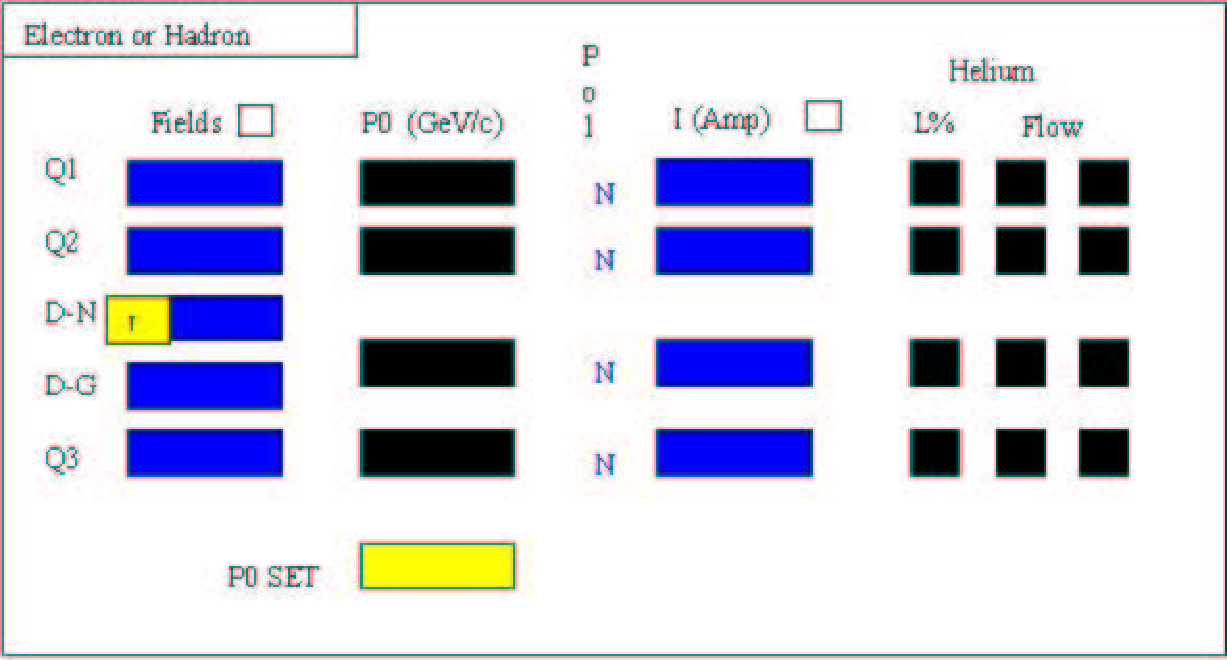
\includegraphics[angle=0,width=15cm,clip]{lerose_cntrl}
{\linespread{1.}
\caption[Spectrometers: Magnet Controls Screen]{Magnet Portion of Main Hall A Control Screen.}
\label{fig:cntrl}}
\end{center}
\end{figure}

This box displays a brief summary of the status of the spectrometer
magnets and their cryogenic systems. The blue fields (with white
numbers) give readbacks of the magnetic fields and currents in each
magnet. The black fields also give readbacks, however in this case if
the text appears green those parameters are OK while if they are red
then that parameter is out of tolerance and may indicate a fault
condition. For example if the helium level goes below a certain point
the magnet will be automatically turned off.  In some cases it may be
desirable to monitor certain critical quantities on a strip chart
(e.g. Magnet settings). A strip chart tool is available for this
purpose from the bottom of the main control screen.

{\bf To set the spectrometers} for a given value of central momentum
(P0) type the desired P0 value into the yellow P0 SET box and hit
return. The magnets will be automatically set to the correct
values. All green numbers in the P0 column indicates that the desired
field or current settings have been reached. 

{\bf Caution:} Re
dipoles, in general it's a bad idea to assume that at the first
instant that the P0 display turns green that the desired field has
been reached and you can start taking data. Stable field is in general
not achieved for from 15 to 30 minutes after reaching the nominal
desired field. This settling time depends on the magnet (Hadron is
slower than Electron) and the magnitude of the field change (small
changes settle faster than big changes). Experimenters are advised to
observe both the field reading and current reading on the magnet in
question and verify that things are stable to their satisfaction
before proceeding.
 
\subsection{ Dipole Field Monitoring Electron Arm}

\noindent (see special instructions for running the Hadron Dipole in field 
regulation mode)

\noindent {\bf Basic Setup}

Each spectrometer dipole magnet is equipped with a Metrolab PT 4025 
NMR Teslameter, several field probes, and multiplexers (to allow switching 
between the probes).  Details of the operation and theory of operation 
for the Teslameter can be found in its user manual, 
a copy of which is available in the the counting house.
The basic layout is shown in Figure~\ref{fig:nmrbasic}


\begin{figure}
\begin{center}
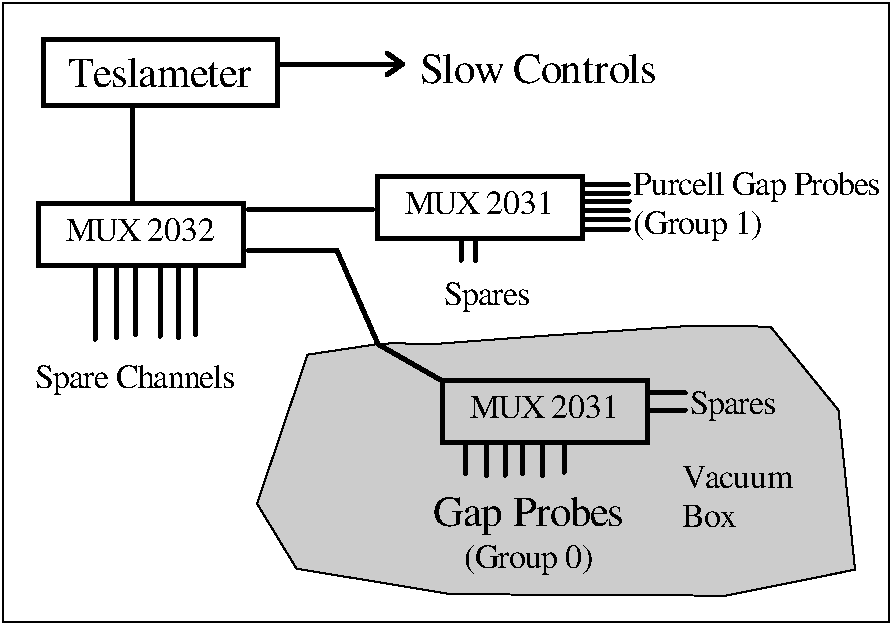
\includegraphics[angle=0,width=15cm,clip]{lerose_fig1}
{\linespread{1.}
\caption[Spectrometers: NMR System Layout]{Basic layout of NMR system}
\label{fig:nmrbasic}}
\end{center}
\end{figure}


 The "Gap Probes" (Group 0 in the controls) are located in two groups 
of three; one group on the low field side of the gap and the other on the high 
field side of the gap.  The groups of three are made up of one each of 
the manufacturer's type 3, 4 \& 5 probes, designed to cover different 
field ranges (see Table \ref{nmr_range}).  The six ``Purcell Gap Probes'' (Group 1 in 
the controls) are located in the Purcell gap of the magnet 
and consists of two each of the above types. {\em Note: Since
the fall of 1998 the multiplexer-multiplexer in the electron arm,
MUX 2032, has been bypassed and hence the ``Purcell Gap Probes'' are currently
unavailable. There are no plans to fix this multiplexer in the
immediate future.}

 The "Gap Probes" are equipped with coils which provide a field 
gradient that cancels out the field gradient of the magnet in the vicinity of 
the probe.  These gradient compensating coils are part of a simple circuit 
that is completely independent of the Teslameter.  The basic circuit for 
the compensating coils is shown in Figure~\ref{fig:nmrcir}


\begin{figure}
\begin{center}
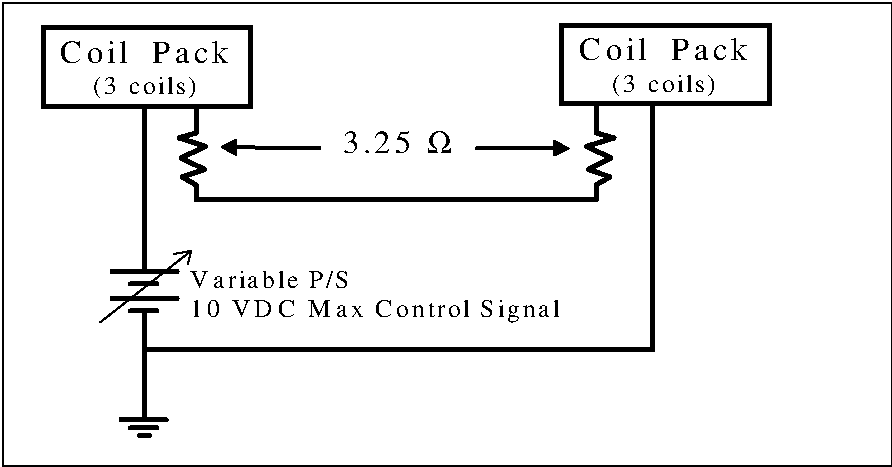
\includegraphics[angle=0,width=10cm,clip]{lerose_fig2}
{\linespread{1.}
\caption[Spectrometers: NMR Gradient Compensation]{Gradient Compensating Circuit.}
\label{fig:nmrcir}}
\end{center}
\end{figure}


%\snfig{figs/lerose_figcce.eps}{Control Voltage calibration for
%Electron Dipole }{nmrcomp4}{5in}

\begin{figure}
\begin{center}
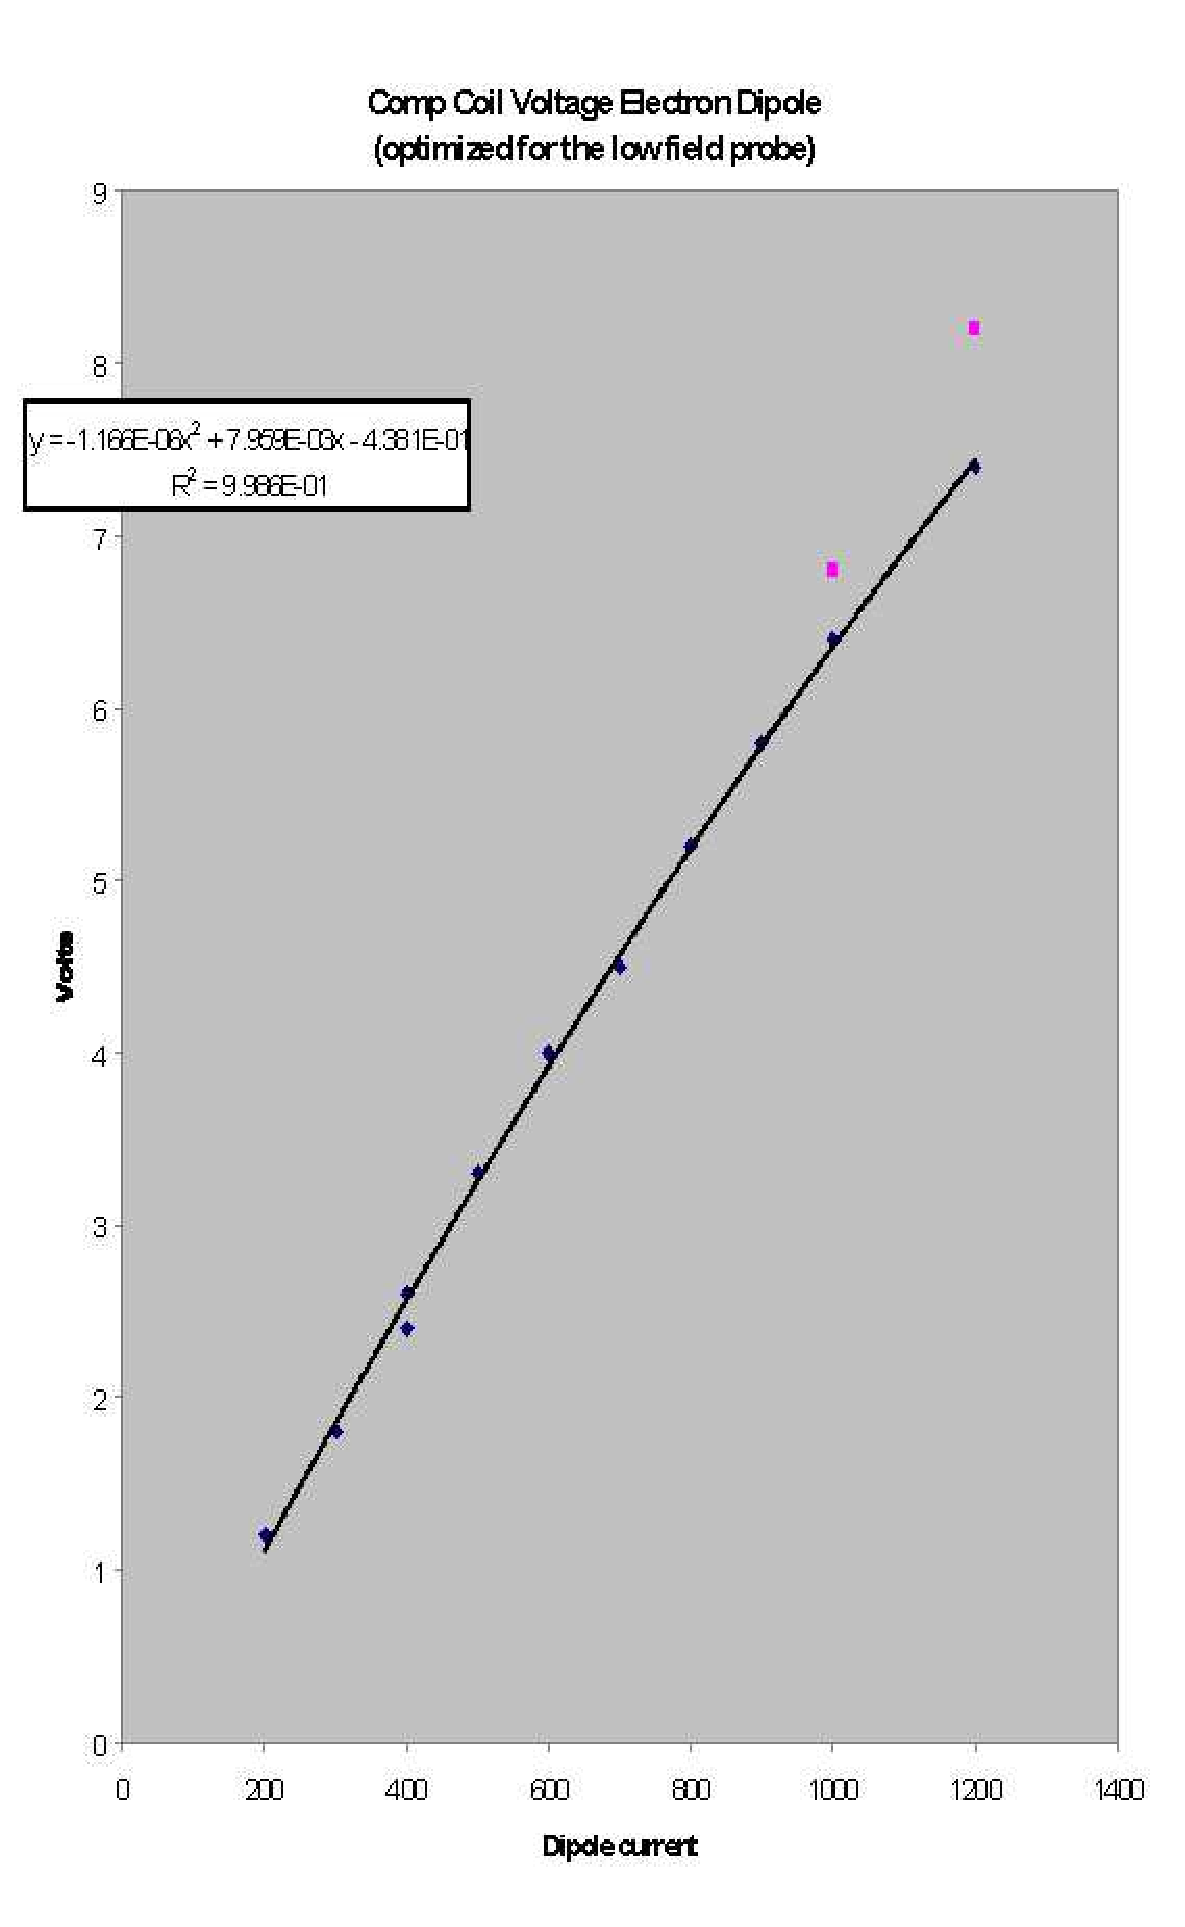
\includegraphics[angle=0,height=20cm,clip]{lerose_figcce}
{\linespread{1.}
\caption[Spectrometers: Control Voltage Calibration for Electron Dipole]{Control Voltage calibration for Electron Dipole.}
\label{fig:nmrcomp4}}
\end{center}
\end{figure}

%\snfig{figs/lerose_figcch.eps}{Control Voltage calibration for
%Hadron Dipole }{nmrcomp5}{5in}
\begin{figure}
\begin{center}
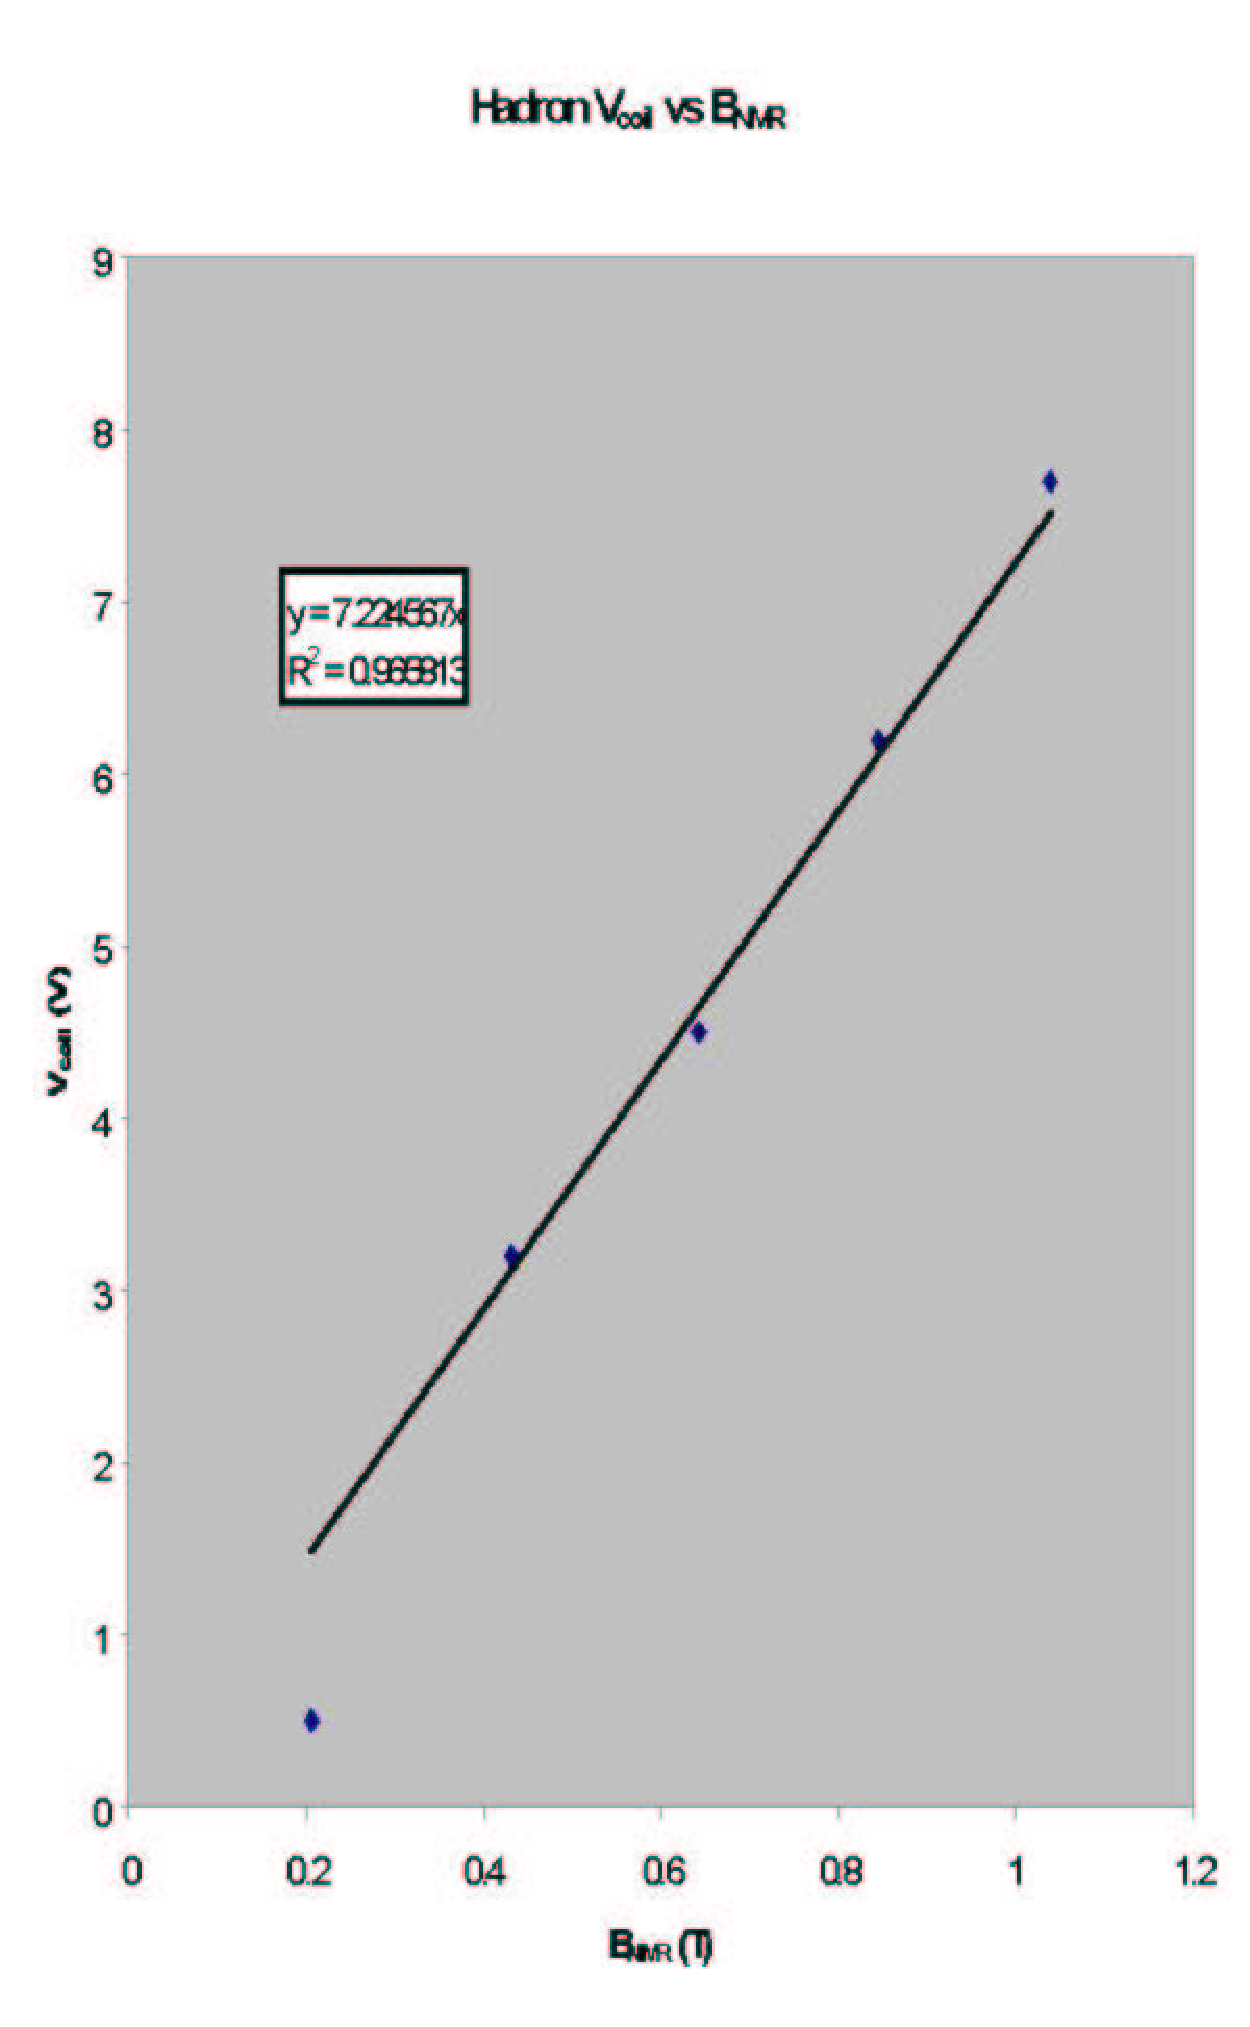
\includegraphics[angle=0,height=20cm,clip]{lerose_figcch}
{\linespread{1.}
\caption[Spectrometers: Control Voltage Calibration for Hadron Dipole] {Control Voltage calibration for Hadron Dipole.}
\label{fig:nmrcomp5}}
\end{center}
\end{figure}

%\snfig{./figs/lerose_fig7.eps}{DAC Calibration for manual operation of NMR probes}{nmr_dac}{9in}
\begin{figure}
\begin{center}
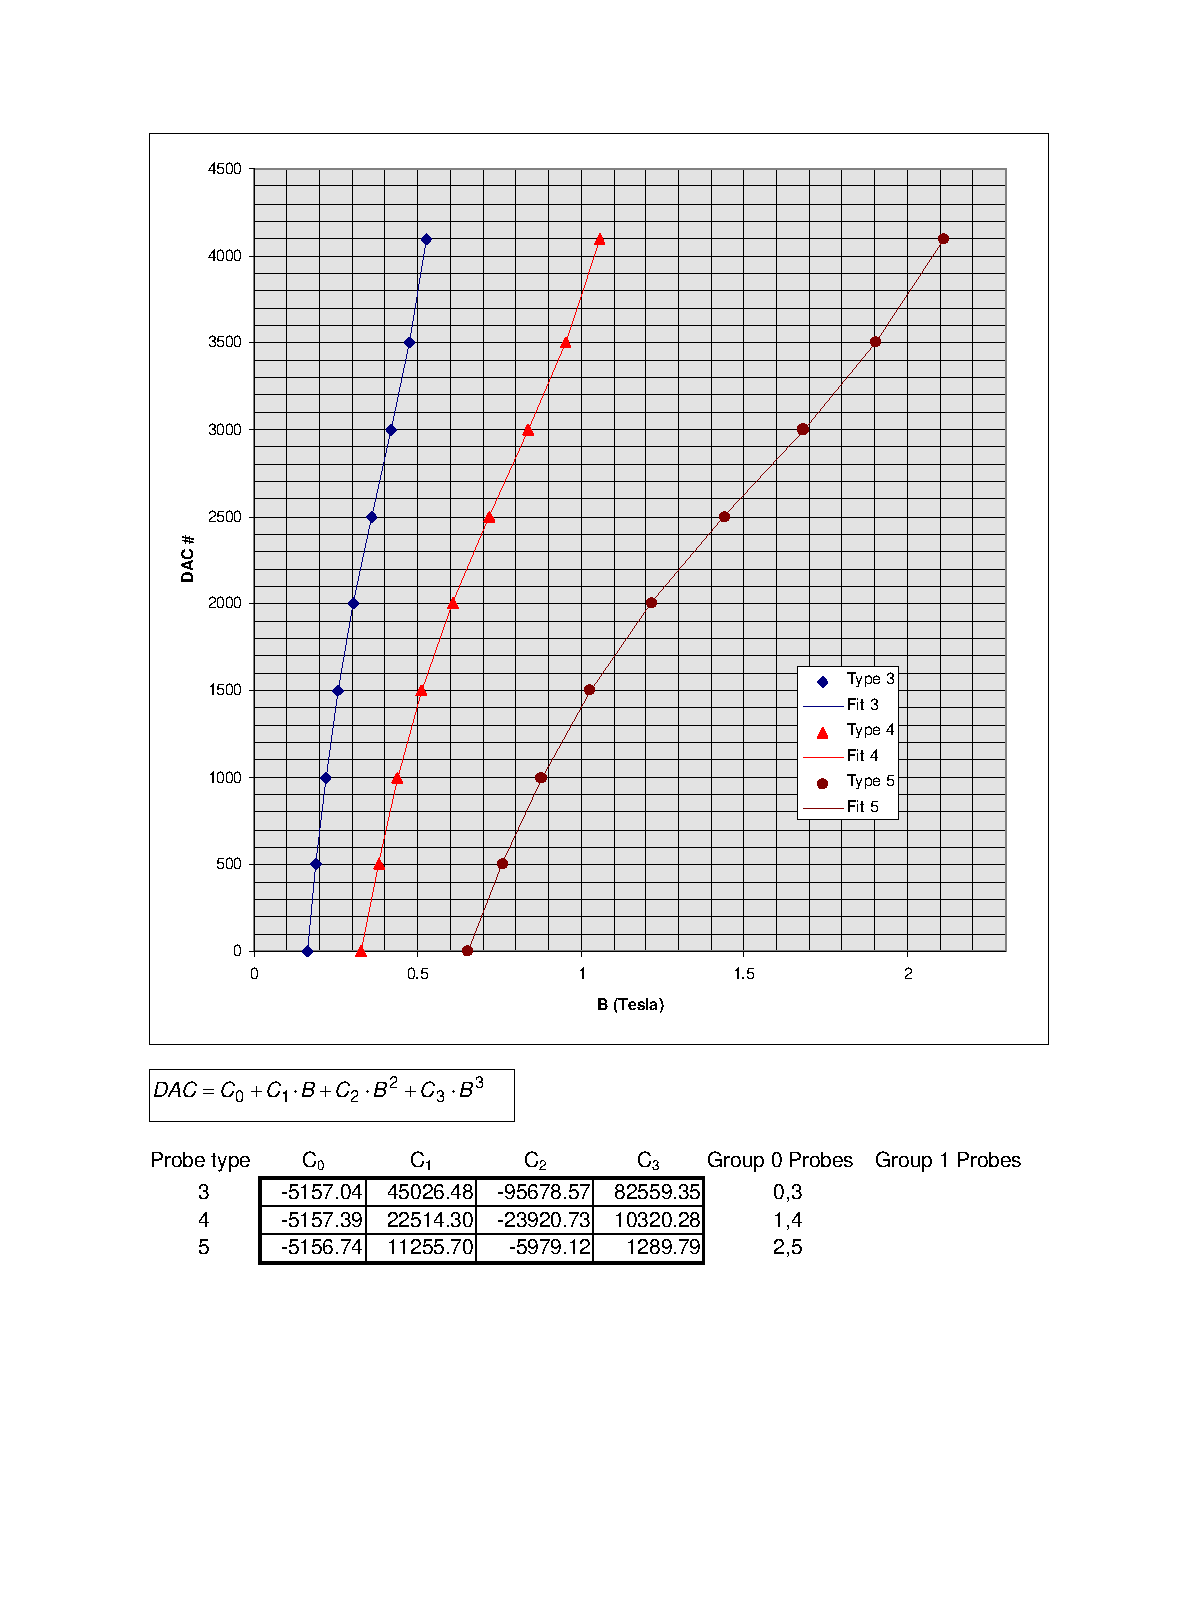
\includegraphics[angle=0,height=20cm,clip]{lerose_fig7}
{\linespread{1.}
\caption[Spectrometers: NMR Probe DAC Calibration]{DAC Calibration for manual operation of NMR probes.}
\label{fig:nmr_dac}}
\end{center}
\end{figure}

The following graphs (see Figures~\ref{fig:nmrcomp4}), 
and ~\ref{fig:nmrcomp5}can be used to determine optimum values for the 
compensating coil control voltage.  It should be noted that the setting 
of the compensating coil current is not very critical in most cases.  In 
general if you're within 10\% of the correct value everything should 
work fine.



\begin{table}
\begin{center}
\begin{tabular}{|cc|} \hline
Probe Type & Field Range (T) \\ \hline 
3 & 0.17 - 0.52 \\
4 & 0.35 - 1.05 \\
5 & 0.70 - 2.10 \\ \hline
\end{tabular}
\caption[Spectrometers: Dipole NMR Probe Field Ranges]{Dipole NMR probe field ranges}
\label{nmr_range}
\end{center}
\end{table}

\subsection{Authorized Personnel}
The following individuals are responsible for NMR operation problems.

\begin{itemize} 
\item[~]J. Gomez - x7498 
\item[~]J. LeRose -x7624
\end{itemize} 

\subsection{NMR Operating Procedure:}

When running in Autopilot mode (see: Simple Spectrometer Field Setting) the 
compensating coil voltage is set automatically and the probe appropriate for 
the field desired is selected. The gaussmeter is placed in SEARCH Mode and the 
dipole power supply regulator is turned on. In this case the dipole current is 
adjusted to achieve the desired field. If the NMR gaussmeter is not "locked" a 
backup Hall Probe is used until the NMR "locks".  The user should just stand 
back and let it work. What follows are instructions for using
the NMR gaussmeter in situations where Autopilot doesn't work or
some special supplemental measurements are required. 

 In principle it is possible to make the field measurements using the 
SEARCH mode in the Teslameter.  In this mode you select a probe and the 
meter explores the whole field range of the probe until it finds and 
"locks" on the resonant signal indicating that it has a field 
measurement.  A "lock" is indicated on the controls display by positive 
field values.  This has the advantage of simplicity but in practice can 
be time consuming and doesn't always work.  The problem being, in 
situations where there is a lot of noise mixed in with the signal, the 
circuitry has problems distinguishing the signal from the noise and gets 
lost before it ever finds a lock.  The problem is exacerbated when the 
field being measured is at the high end of the probe's range.  In this 
case the search starts at the low end and keeps getting hung up on the 
noise and never gets to the field range of interest.  The solution to 
this problem is to tell the device approximately what field it's looking 
for and use the AUTO mode to find the lock.  In the procedure below that 
is what we will be doing.

In any case, for "gap probes" (group 0) you must energize and adjust 
the gradient compensating coils for the field ranges to be measured before 
trying to make measurement.

For studies involving 
10\% changes in the field settings the compensating coil current can be 
set once and left alone.


\noindent\underline{\bf Recommended Procedure:}(turn the {\bf REGULATOR OFF} for all 
non-autopilot field measurements)\\
For group 0 probes set compensating coils appropriately (see figures).\\
Put meter in MANUAL mode with SEARCH OFF \\
Select a probe \underline{\bf and} polarity (\underline{\bf Group 0:  
Probes 0, 1, 2 negative;} {\underline Probes 3, 4, 5 positive}) \\
Type in DAC number for the field range being measured (see below) \\
Select AUTO and wait for a lock (positive field reading) \\
Verify that you have a good lock by checking the oscilloscope for a 
clear resonant signal. \\
Go back to 2. for the next probe \\
If you have problems see the table listing problems and possible 
solutions.

\noindent\underline{\bf Selecting DAC \#'s}

In selecting the DAC \# to use for the field of interest use 
either the graph in Figure~\ref{fig:nmr_dac} or the polynomial below that.

\pagebreak
\noindent{\bf Problems and Solutions}\\

\begin{tabular}{|l|l|}\hline
Symptom & Diagnosis and Cure \\ \hline\hline
Weird numbers on displays, controls for & Need to reboot.  \\
all magnets fouled up & See instructions below. \\ \hline
NMR Teslameter does not respond to  & Meter's communications are \\
& somehow hung up. \\
commands and display shows all zeros. 
& Push {\bf RESET}. \\  
&  \\ \hline
Will not lock & Very high noise level \\ 
& makes resonance hard to find. \\
Still will not lock & Very high noise level makes \\
& resonance hard to find.  Search \\
& for the resonance manually by \\
& adjusting the DAC in manual \\
& mode until you see the resonant \\
& signal.  (It helps if you know \\
& what field you expect so you'll \\
& know where to look). \\ \hline
You find resonance manually & Check probe polarity. \\
but still can't get a lock & Try decreasing and \\
& increasing DAC number by 1. \\
& Optimize signal by adjusting \\
& compensating coils. \\ \hline
Can't find resonance manually & Try a different probe.  Use \\
& readings from other probes to \\
& tell you where to look for \\
& the resonance with the probe \\
& that's giving you trouble. \\
& Make sure compensating coils are \\
& energized properly. \\
& Make sure magnet is on. \\ \hline\hline
\end{tabular}

\vskip.5cm
\paragraph{\bf Hadron Dipole Field Setting Instructions:}

Turn on power supply (contact Mark Stevens, John LeRose, 
or Javier Gomez for assistance).\\


Turn on field regulation mode. Type desired field value into FieldSet 
(yellow field). Wait for field to reach the desired value (read from the blue 
field). After reaching the desired field wait 15 minutes to assure stable field.
Pay attention to the current and field readings.
{\bf If} the NMR is locked, (the NMR is locked if the field reading in 
the blue field has a positive number and is updating itself), don't 
worry it will get there.\\

{\bf If} the NMR is not locked (negative but updating number in the blue 
field) {\bf but} the current appears to be going in the right direction, 
 don't worry it will get there and the NMR should lock when you get into 
the vicinity of the desired field.  If you're worried anyway and want to 
watch the field change, push SEARCH.  (The NMR will search over the 
full range of the probe rather than just in the vicinity of the desired 
field.)  The NMR should lock in a minute or two.\\

{\bf If} the NMR is not locked {\bf and} the current is going in the 
wrong direction (This can happen if you ask for a new field before you 
reach a stable setting), you {\bf must} push SEARCH.  (The NMR will 
search over the full range of the probe rather than just in the vicinity 
of the desired field.)  The NMR should lock in a minute or two and the 
software will correct the current setting appropriately but slowly.  If 
the NMR doesn't lock you may have to ask for a field value appropriate 
for the present current ($\sim$ 1.1 $\times$ 10$^{-3}$ T/Amp).  The NMR 
will only search in the limited region of the requested field and should 
find a lock more easily.  After getting the lock let things settle in 
for a few minutes and then ask for the field you want again.  In extreme 
cases you may have to nurse it through the transition by asking for 
multiple small increments.  If you ask for a change of less than 5\% the 
NMR should not lose its lock.\\

\noindent To shut down:  Set FieldSet to .18.  Let current run down to 
just over 100 Amps.  Then push stop on Dipole control screen\\

\begin{table}[ht]
\begin{center}
\begin{tabular}{|l|l|l|}\hline
Problems & Explanation & Action \\ \hline
NMR not locked but  & Normal operation for  & Wait. (see 
above) \\ 
current is changing in & large field & \\ 
the right direction & changes  & \\
 && \\ \hline
NMR locked but current & Normal operation. & Wait. \\
going in the wrong & & \\
direction. & & \\ \hline
NMR locked but field not & Field regulation is & Check 
that field regulation \\
correct and current not & disabled  or software & is enabled.  Enter 
desired \\
changing & is confused. & field value or one \\
&& very near the \\
&& desired value again. \\ 
  &  & \\
\hline
NMR field display freezes. & NMR Gaussmeter is not & Push {\bf RESET}. \\
(Usually but not always & communicating with &  \\
shows  -\#.0000000) & software. & \\ \hline
\end{tabular}
\end{center}
\caption[NMR troubleshhoting]{NMR troubleshhoting
}
\label{tab:hrs_nmr_2}
\end{table}

\subsection{Powering Up Dipole Magnets:}
\noindent
Use these instructions to recover from loss of a magnet due to a fault
(e.g. He level or lead flow fault). The order of actions matters. \\
(Contact Tech on call if anything behaves funny or things don't
respond as expected. Sometimes after a trip an access to the Hall is
required to reset things)\\

\noindent 1. Wait for Iout=0 (you can't and don't want to do anything while the magnet is in emergency fast dump mode.)\\
\noindent 2. While waiting, make a log entry re the fault. Give details such as time, coincident activities, and nature of the fault.\\
\noindent 3. Make sure the fault is cleared. (e.g. He level and flow rates returned to normal values and stable)\\
\noindent 4. In the HRS Hadron (Electron) Dipole Systems' control panel:\\
\noindent(a) Press RESET (verify that all faults are cleared in the middle column)\\
\noindent(b) Press START (Display will indicate Power Supply ON and magnet ENGAGED)\\

Power supply and magnet are ready to go. From here you can return
to "Autopilot Mode" 
(type in desired P0 on control screen and wait) or proceed as described below.
For Electron dipole type in desired current in I Set and the power supply will respond.\\ 
For Hadron dipole go to HRS HADRON DIPOLE NMR control panel.\\

\noindent 1. Press RESET\\
\noindent 2. Press Reg. Enable YES\\
\noindent 3. Press Search ON (should already be on but it doesn't hurt to check)\\
\noindent 4. Type desired field into Field Set (T) field.\\
\noindent 5. Wait for field to reach the desired value. (In general it's a good idea to wait about 15 minutes after first reaching
 the desired field before taking data.) See Hadron Dipole Field Setting for more details and help with trouble shooting.\\

\subsection{Starting Q1 Power Supply:}
\noindent Do this when a fault causes the power supply to shut off.\\
\noindent Wait for fault to clear (watch He levels). \\
\noindent 1. Push RESET (check all faults cleared)\\
\noindent 2. Select desired polarity\\
\noindent 3. Push ON\\
\noindent 4. Type in ISET (yellow field) or re-enter P0 in Autopilot Mode.\\

\subsection{Starting Q2/3 Power Supply:}
\noindent Do this when a fault causes the power supply to shut off.\\
\noindent 1. Wait for cause of fault to clear (e.g. low Helium level)\\
\noindent 2. Press RESET\\
\noindent 3. Select polarity\\
\noindent 4. Press ON\\
\noindent 5. Type in ISET (yellow field) or re-enter P0 in Autopilot Mode.\\
} %infolev
% ===========  CVS info
% $Header: /group/halla/analysis/cvs/tex/osp/src/hrs/nmr-1999.tex,v 1.2 2003/12/05 06:49:07 gen Exp $
% $Id: nmr-1999.tex,v 1.2 2003/12/05 06:49:07 gen Exp $
% $Author: gen $
% $Date: 2003/12/05 06:49:07 $
% $Name:  $
% $Locker:  $
% $Log: nmr-1999.tex,v $
% Revision 1.2  2003/12/05 06:49:07  gen
% infolevels added, polishing
%
% Revision 1.1  2003/06/06 15:44:08  gen
% Revision printout changed
%
% Revision 1.2  2003/06/05 23:30:00  gen
% Revision ID is printed in TeX
%
% Revision 1.1.1.1  2003/06/05 17:28:31  gen
% Imported from /home/gen/tex/OSP
%
%  Revision parameters to appear on the output
